\section{Discussion \& Conclusion}
	\begin{enumerate}
		\item The NPN characteristics graph showed expected results, with the collector current remaining constant for a given base current, independent of the collector voltage above the threshold voltage of the Base-collector region.
		\item The Multi-vibrator graph also matched the expected behavior in both cases, although there were slight errors in observed frequency and duty cycle values due to resistance and capacitance tolerances.
		\item The EM wave graph exhibited two opposite peaks at different times, with the second peak being larger than the first peak. This indicates that the induced emf depends on the velocity of the magnet, with a higher moment of the magnet resulting in a larger emf. Negligible effects from Lenz's law and buoyant force were observed, and the magnetic moment of the magnet was calculated to be $(8.79\pm 0.12)$ Am$^2$.
		\item We were able to estimate the acceleration due to gravity using a rod pendulum and a phototransistor, chich came out to be remarkably close to the literature value, $g=(9.728\pm 0.005)$ m/s$^2$. Let us also note that $g$ can slightly vary from place to place.
		\item We were also able to observe sound beats produced by the superposition of two sound waves of nearl equal frequencies. The sound and beat frequencies were observed to be $f=3448.2$ Hz and $f_b=98.1$ Hz respectively, which are about 0.001\% and 0.02\% deviated from the theoretical values.
	\end{enumerate}

\section{Precautions and Sources of Error}

    \begin{enumerate}
        \item For the rod pendulum, the length is measured from the knife edge to the bottom and used in the
		formula. But there is a small mass projecting above the knife edge that is not included in the calculation.
		Also the calculations assume that the pendulum must be exactly vertical in the resting position, which
		has to be ensured.
		% \item Make sure that the magnet is not damaged when falling from a height.
		\item Make sure that the amplitudes of the two sound waves are nearly equal.
    \end{enumerate}

% \vspace{-3em}
\appendix
\section{Screenshots from the Software}

\begin{figure}[H]
	\centering
	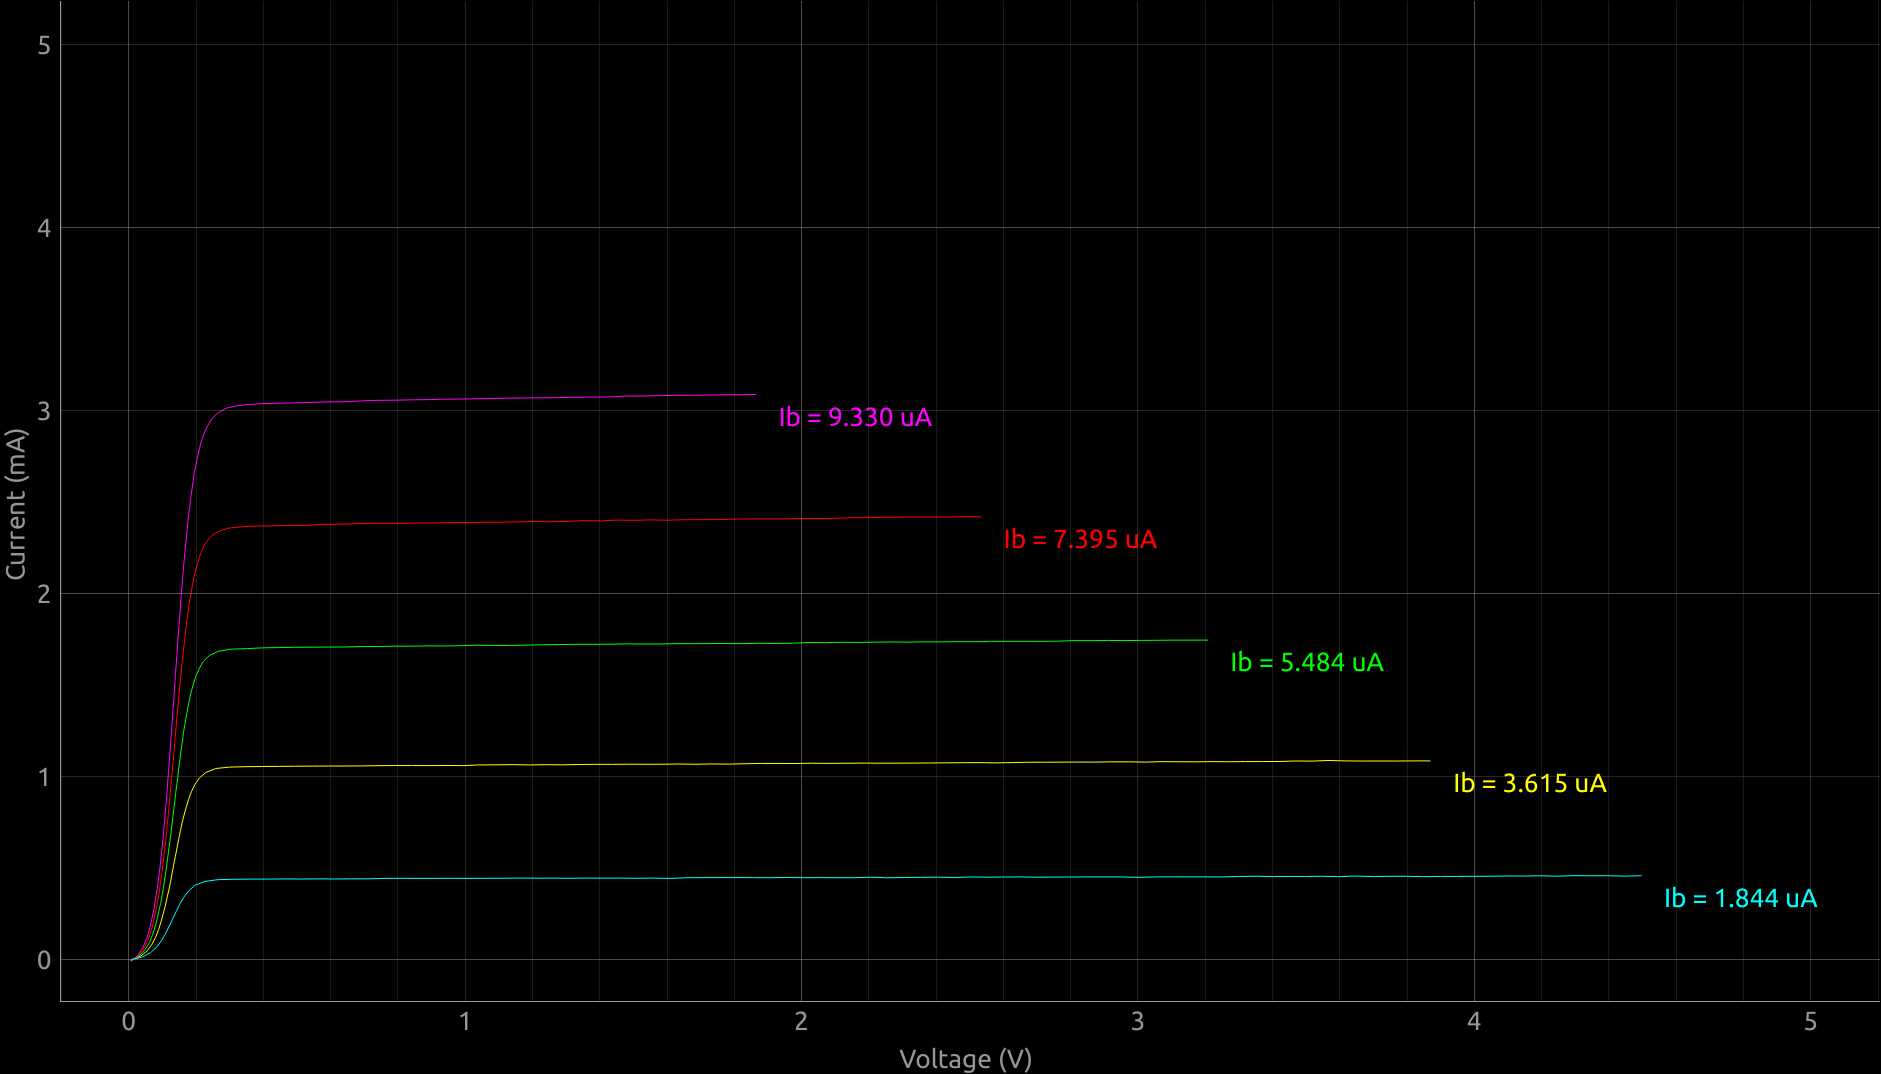
\includegraphics[width=1\columnwidth]{data/npn.png}
	\caption{NPN characteristics}
\end{figure}

\begin{figure}[H]
	\centering
	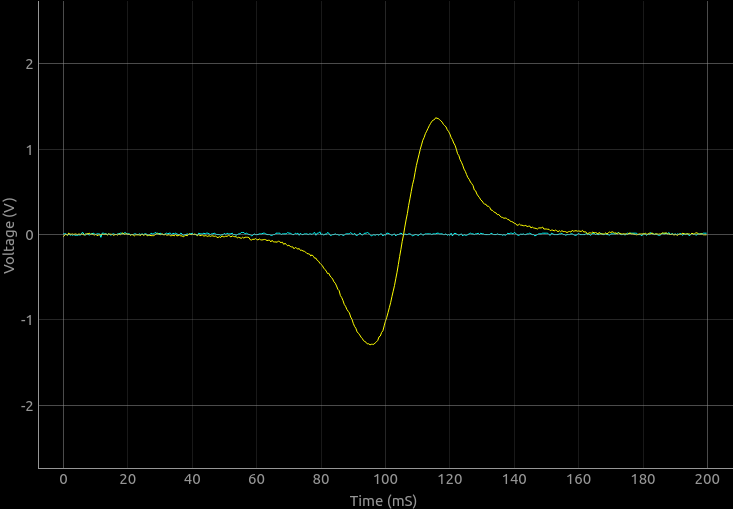
\includegraphics[width=1\columnwidth]{data/m.png}
	\caption{emf produced by a falling magnet on a coil}
\end{figure}

\begin{figure}[H]
	\centering
	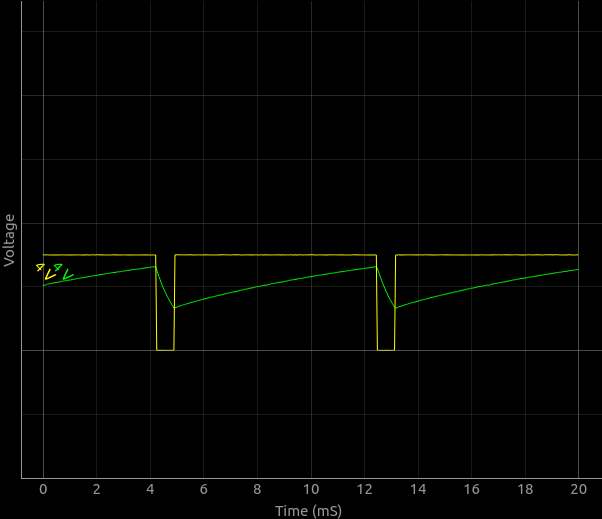
\includegraphics[width=1\columnwidth]{data/5552.png}
	\caption{Astable Multivibrator}
\end{figure}

\begin{figure}[H]
	\centering
	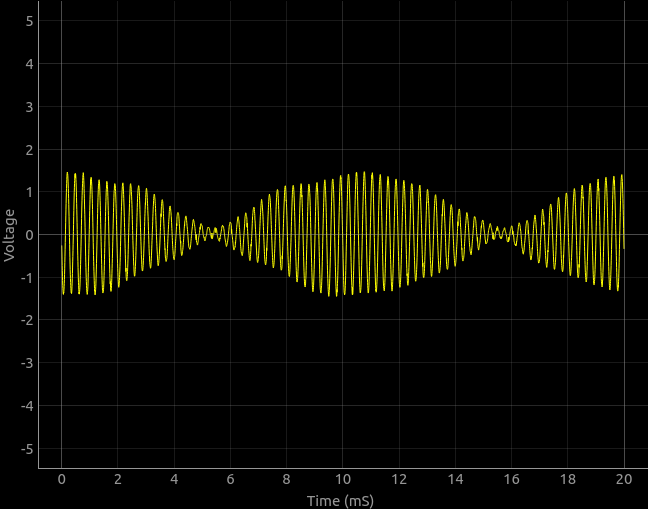
\includegraphics[width=1\columnwidth]{data/beats.png}
	\caption{Beats produced by two sound waves of nearly equal frequencies}
\end{figure}